\documentclass[tikz]{standalone}
\usepackage{pgffor}

\begin{document}
    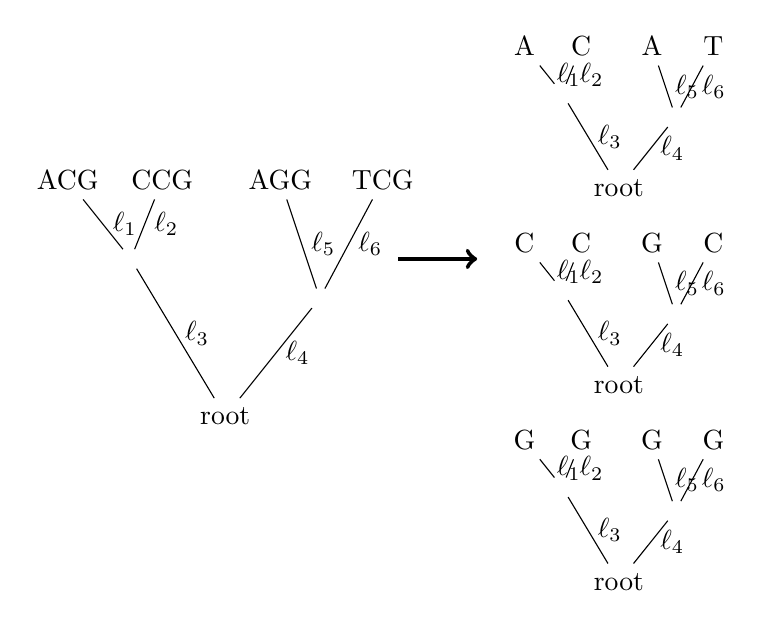
\begin{tikzpicture}
        \foreach \x/\y/\n/\l/\j/\k in {-2/2/a/A/C/G,-0.8/2/b/C/C/G,0.7/2/c/A/G/G,2/2/d/T/C/G}{
            \node[] (\n) at (\x,\y) {\l\j\k};
            \node[] (\n1) at (5+0.6*\x,2.5+0.6*\y) {\l};
            \node[] (\n2) at (5+0.6*\x,0.6*\y) {\j};
            \node[] (\n3) at (5+0.6*\x,-2.5+0.6*\y) {\k};
        }
        \foreach \x/\y/\n/\l in {-1.2/1/lnode/,1.2/0.5/rnode/,0/-1/r/root}{
            \node[] (\n) at (\x,\y) {\l};
            \node[] (\n1) at (5+0.6*\x,2.5+0.6*\y) {\l};
            \node[] (\n2) at (5+0.6*\x,0.6*\y) {\l};
            \node[] (\n3) at (5+0.6*\x,-2.5+0.6*\y) {\l};
        }
        \foreach \m/\n/\l in {a/lnode/{$\ell _1$},b/lnode/{$\ell _2$},c/rnode/{$\ell _5$},d/rnode/{$\ell _6$},lnode/r/{$\ell _3$},rnode/r/{$\ell _4$}}{
            \draw[] (\m) -- node[right]{\l} (\n);
            \draw[] (\m1) -- node[right]{\l} (\n1);
            \draw[] (\m2) -- node[right]{\l} (\n2);
            \draw[] (\m3) -- node[right]{\l} (\n3);
        }
        \draw[ultra thick, ->] (2.2,1) -- (3.2,1);
    \end{tikzpicture}
\end{document}